% --- Hidden Markov Models 
\begin{tikzpicture}
    \node [mybox] (box){
        \begin{minipage}{0.48\textwidth}
            \begin{center}
                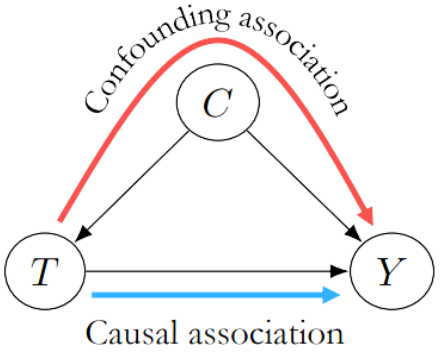
\includegraphics[width=0.48\textwidth]{imgs/07_example.png}
            \end{center}
            
        \begin{tabular}{lp{0.48\textwidth} l}
            Individual treatment Effect (ITE) & 
            $  
                ITE_{i} = Y_{i}(1) - Y_{i}(0)
            $

            $
                \begin{cases}
                    ITE_{i} = 1 \ \text{if there is causal association} \\
                    ITE_{i} = 0 \ \text{otherwise}
                \end{cases}
            $
            
            \\

            Average treatment effect (ATE) & 
            $  
                \mathbb{E}[Y_{i}(1) - Y_{i}(0)] = \mathbb{E}[Y_{i}(1)] - \mathbb{E}[Y_{i}(0)]
            $
            
            $
                \neq \mathbb{E}[Y | T = 1] - \mathbb{E}[Y | T = 0]
            $

            $i$ is the same individual!
            \\

            Randomized Control Trial (RCT) & 
            \parbox[t]{0.48\textwidth}{
                randomizes subject into treatment groups
                to remove confounding association.

                In this case, 
                \begin{center}
                    $ATE = \mathbb{E}[Y | T = 1] - \mathbb{E}[Y | T = 0]$
                \end{center}
            } \\

            Observational Study & 
            observes subjects in their natural environment
            without randomization.

            \\

            Adjust for confounding  &
            
            Shield all the paths from $T$ to $Y$
            In this case, even if no RCT:
            \begin{center}
                $
                    \mathbb{E}[Y(t) | W = w] =
                $

                $
                    = \mathbb{E}[Y | do(T = t), W = w]
                $

                $
                    = \mathbb{E}[Y | T = t, W = w]
                $
            \end{center}
            \\

            Backdoor adjustment example &

            $
               \mathbb{E}[Y|do(T=t)] =
            $

            $
               = \mathbb{E}_{C} \mathbb{E}[Y|t,C] 
               = \sum_{c \in C} \mathbb{E}[Y|t,c] P(c)
            $


        \end{tabular}    \end{minipage}
};
%------------ Hidden Markov Models Header ---------------------
\node[fancytitle, right=10pt] at (box.north west) {Causal Inference};
\end{tikzpicture}